\section{Overview}
Our approach proposed in this paper is shown in \figref{fig:stepMap}. We divide our approach into two main parts: off-line work and runtime execution.
\begin{figure}[H]
	\centering
	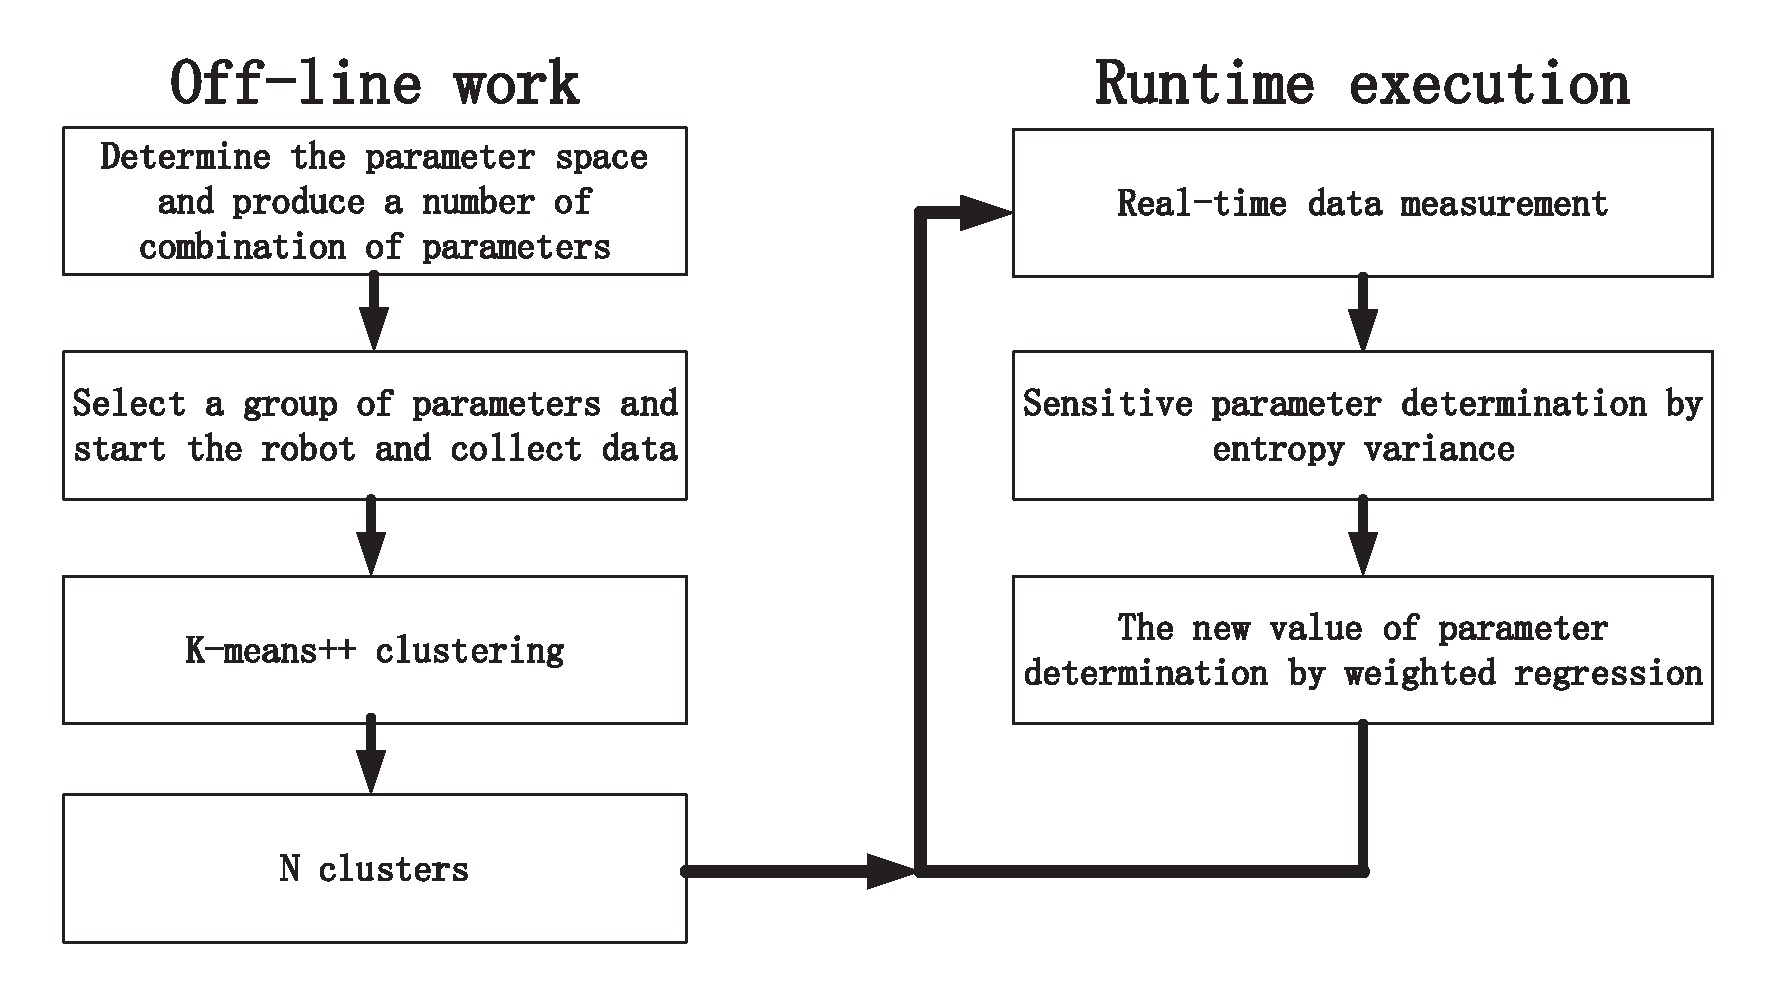
\includegraphics[width=1.0\linewidth,height=140pt]{fig/mainwork/stepMap}
	\caption{The overall approach}
	\figlabel{fig:stepMap}
\end{figure}

In off-line work, firstly, we define parameter space and let the robot climb the poles with different diameters by different parameters which are stable during climbing. When the robot are climbing the pole, we record the velocity and joint angles of the robot every two seconds. After that, we combine all the data from climbing different poles together and then conduct clustering~\cite{Cluseter_ICT,KmeansAndDeepLearning} on the whole data.

In runtime execution, we will collect the real-time data like joint angles,  velocity and the value of parameters every two seconds and then select the  data recorded in off-line work to our calculation by clustering the real-time data. After selecting the data we need, we determine the parameter whose change has the greatest effect on the motion of the robot by entropy variance. And finally we get the new value of the selected parameter by weighted regression. 

Currently, a widely used of control strategy for snake-liked robots is based on the sinusoidal motion model~\cite{HiroseSine} which is proposed by professor Hirose. After that, Tesch et al. proposed a parametric equation based on the sinusoidal model for a snake-liked robot with three-dimensional athleticism~\cite{ChosetSine}. This parametric equation simplifies the control strategy of the snake-like robots and allows the robot to determine the motion model of the machine with a small amount of control parameters. We take rolling gait~\cite{Enner2013Motion} as our climbing gait in simulation. The sinusoidal motion model function about rolling gait is shown in the following formula:
\begin{eqnarray}\label{basicRoll}
T_i=\left\{
\begin{array}{lr}
A\cdot \sin (\omega \cdot t + i\cdot \varepsilon )&odd\\
A\cdot \sin (\omega \cdot t + i\cdot \varepsilon +  \frac{\pi}{2})&even
\end{array}
\right.
\end{eqnarray}

By modifying the amplitude $A$, phase $\varepsilon$, and angular rate $\omega$ in Eq.\ref{basicRoll}, the maximum rotation angle of joints, robots' shape and the motion rate of the snake-liked robot are changed. Unlike the biological snake, rolling gait can be performed by snake-liked robot. Rolling gait is an easy but effective gait. Snake-liked robot can move on the ground or climb the pole by rolling gait with suitable parameters.
